\chapter{Détecteurs basés sur l'ionisation des gaz}
\section{Principes généraux d'un détecteur à gaz}
Lorsqu'une particule chargée traverse un gaz, elle excite et ionise des molécules le long de son
parcours. L'ionisation se résulte par l'apparition d'une paire d'ion forme de l'électron libre et
de l'ion positif. Nous avions vu que le nombre $N_i$ de paires d'ions créées s'obtient via
\begin{equation}
N_i=\frac{E_{abs}}{W}
\end{equation}
S'il n'y a pas de mécanisme de collection par diffusion des paires et par multiples collisions 
thermiques, elles retrouvent vite l'énergie thermique et se recombinent. En appliquant un champ 
électrique entre deux électrodes les ions se dirige vers elles. Cette accélération peut être
interrompue après chaque collision mais le champ, toujours présent, les ré-accélère ensuite vers
les électrodes. Dès lors, bien que le signal soit microscopiquement chaotique, à l'échelle 
macroscopique les charges dérivent à vitesses constante dans la direction du champ : la tendance
est d'aller tout de même dans une certaine direction et il en résulte un signal mesurable.\ \\

\exemple{Une particule chargée de 1 MeV crée environ 30 000 paires d'ions. Cela correspond à une 
charge collectée de $5*10^{-15}$ C. Pour un détecteur avec une capacité standard de 30 pF, 
l'amplitude du signal mesuré vaut environ 0.15 mV.}

\subsection{Dépendance dans l'intensité du champ électrique}
On peut séparer le comportement par \textit{régions} (voir graphique ci-dessous).





	\subsubsection{Région I}
	Lorsque le champ est nul, rien n'est connecté à cause des recombinaisons. Lorsque la tension
	augmente, ces forces sont dominées (les charges sont plus écartées) ce qui rend le processus
	plus efficace : de plus en plus de paires sont collectées. Ceci n'a pas contre pas d'utilisation
	pratique.
	
	\subsubsection{Région II}
	On arrive ensuite à un certain seuil où toutes les charges crées sont collectés (augmenter la
	tension n'a plus d'effet). Un détecteur fonctionnant dans cette région collecte directement 
	les ionisations produites, il s'agit d'une \textbf{chambre d'ionisation}. Comme le signal est
	très faible on utilise ces chambres pour des mesures d'exposition de $\gamma$, généralement en
	mode courant.
	
	\subsubsection{Région III}
	En augmentant la tension, le nombre de charge collecté augmente et on se retrouve sur un flanc
	montant entre deux paliers : c'est la $3^e$ région. L'augmentation des charges vient du fait que
	le champ est assez intense pour accélérer les ions libérer jusqu'à une énergie qui leur permet
	aussi d'ioniser les molécules du gaz. Les ions secondaires peuvent produire encore plus 	
	d'ionisation. C'est le phénomène d'\textit{avalanche} qui est directement proportionnel au 
	nombre d'électron primaire (on observe en effet un rapport linéaire avec le nombre de paires
	dans cette zone). Un détecteur opérant dans cette région est un \textbf{compteur proportionnel}.\\
	
	\textsc{Remarque}\ \\
	L'ionisation \textit{primaire} est celle produite par la particule incidente et toutes les 
	secondaires mises en mouvement tandis que la \textit{secondaire} est celle produite par les
	particules secondaires.
	
	\subsubsection{Région IV}
	Si la tension augmente encore, on se retrouve à la fin du flanc montant où la cascade est si
	importante qu'il y a des distorsion à l'anode causant la perte de proportionnalité. Aucun 
	détecteur n'opère dans cette région.

	\subsubsection{Région V}
	A partir d'une certaine tension, l'énergie est si grande que des décharges se produisent dans 
	le gaz. Même si la probabilité est faible, le nombre est tellement important qu'un UV émis par 
	la désexcitation des molécules va interagir avec le détecteur et le saturer : l'amplitude 
	est identique indépendamment de l'énergie de la particule incidente. Il n'est donc plus possible
	de faire de la sepctro, mais simplement du comptage. Ces détecteur sont les \textbf{compteurs
	Geiger-Müller}. Cette région est caractérisée par un plateau pour lequel le signal varie peu.
	
	\subsubsection{Vers la région VI et au delà!}
	Une décharge continue se produit mais il faut éviter pour éviter d'endommager le compteur.\\
	
	Il n'existe donc \textbf{pas} de détecteur "universel" opérant dans toutes les régions de 
	tension, chaque type de détecteur à gaz possède ses propres caractéristiques (géométrie, type, 
	\dots). Le schéma montré ci-dessus n'est pas possible, on ne peut donc pas "simplement" régler 
	la tension et choisir son mode de fonctionnement.
	
	\begin{center}
	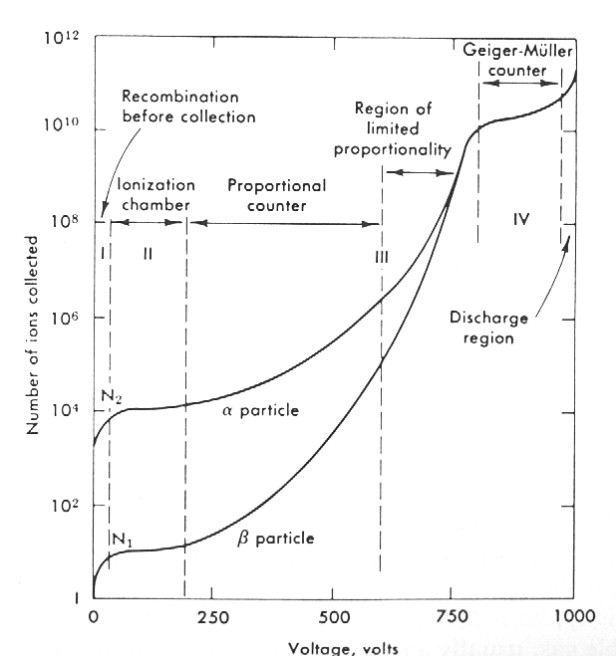
\includegraphics[scale=0.3]{ch8/image1}
	\captionof{figure}{L'échelle de tension (abscisse) est arbitraire}
	\end{center}
	
\section{Transport des charges dans un gaz}%sl15	
	\subsection{Diffusion}
		\subsubsection{Collisions dans un gaz à l'équilibre}
		Dans un gaz, les atomes neutres/molécules sont en constante agitation thermique dont la
		distribution (ndlr. des vitesses) est donnée par la distribution de 
		\textsc{Maxwell-Boltzmann}
		\begin{equation}
		f(\vec{v})d\vec{v}=\left( \frac{m}{2\pi kT}\right)^{3/2}\exp{(-mv^2/2kT)}d\vec{v}
		\end{equation}
		où $k=1.38*10^{-23}$ J.K$^{-1}$, $T$ la température (K) et $m$ lamasse de la particule. La
		vitesse moyenne $\langle v\rangle$ vaut
		\begin{equation}
		\langle v\rangle=\sqrt{\frac{8kT}{\pi m}}
		\end{equation}
		Pour des électrons à température ambiante, $\langle v_{e^-}\rangle \approx 10^5$ m.s$^{-1}$.
		Pour des ions d'Ar $\langle v\rangle \approx 370$ m.s$^{-1}$ soit un facteur 100 a 1000 
		(en général) de différence.
		
		
		\subsubsection{Section efficace et libre parcours moyen}
		Un gaz parfait n'étant composé que d'une seule espèce de molécules, on peut y déterminer 
		la probabilité par unité de temps qu'une molécule subisse une collision avec une autre, 
		on retrouve une formule bien connue
		\begin{equation}
		\tau^{-1}=\langle v_r\rangle\sigma_0 N
		\end{equation}				
		où la section efficace de collision $\sigma_0$ est constante, $N$ est la densité et 
		$\langle v_r\rangle$ est la vitesse relative entre les deux particules. Celle-ci est 
		donnée par la différence des vitesses relatives
		\begin{equation}
		\overrightarrow{v}_r=\overrightarrow{v}_A-\overrightarrow{v}_B \Rightarrow \langle
		 v_r^2\rangle=\langle v_A^2+v_B^2-2\overrightarrow{v}_A\overrightarrow{v}_B\rangle
		\end{equation}
		Ces vitesses étant aléatoires, le produit scalaire est en moyenne nul. Dès lors
		\begin{equation}
		\langle v_r\rangle = \sqrt{2}\langle v\rangle
		\end{equation}
		Le temps $\tau$ est ainsi l'intervalle de temps moyen entre deux collisions d'une 
		molécule dans un gaz à l'équilibre thermodynamique. Si cet équilibre est perturbé, il 
		se rétablit après un certain temps de relaxation dépendant de $\tau$, mais ceci est plus 
		informatif. Le libre parcours moyen - distance moyenne entre deux collisions pour une 
		molécule dans le gaz - s'obtient via
		\begin{equation}
		\lambda=\langle v \rangle\tau=\frac{1}{\sqrt{2}\sigma_0 N}
		\end{equation}
		Comme $N=f(P)$, $\lambda$ dépend de la densité et de la pression. A l'échelle atomique, les
		collisions sont relativement peu fréquentes ($\lambda(Ar) \approx 6.12*10^{-8}$ m.

		\subsubsection{Diffusion en l'absence de champ électrique}
		Afin d'introduire le coefficient de diffusion $D$, il est nécessaire de discuter de ce cas.
		Sans champ électrique, les paires créées interagissent avec les molécules de gaz et cèdent
		leur énergie jusqu'à être thermaliser à $kT\approx0.025$ eV. Ces paires sont créées le 
		long de la trajectoire (rectiligne) et vont diffuser par rapport à cette ligne. Elles vont
		ensuite diffuser selon une distribution gaussienne. En 3D :
		\begin{equation}
		dN(\overrightarrow{r})=\frac{N_0}{(4\pi Dt)^{3/2}}\exp{\left(-\frac{r^2}{4Dt}\right)}
		d\overrightarrow{r}
		\end{equation}
		où $D$ est le coefficient de diffusion (m$^2$.s$^{-1}$)qui dépend de la charge, du gaz, 
		de $T$, \dots Dans le cas à une dimension
		\begin{equation}
		dN(x)=\frac{N_0}{(4\pi Dt)^{1/2}}\exp{\left(-\frac{x^2}{4Dt}\right)}dx
		\end{equation}
		Distribution dont la variance $\sigma^2=2Dt$ augmente lorsque $t$ augmente.
		
	\subsection{Transport des particules}%sl25
	Sous l'application d'un champ électrique, les ions se déplacent vers la cathode et les électrons
	vers l'anode. Ces mouvement migratoires se superposent au mouvement thermique ainsi que les 
	collisions avec les molécules de gaz : il faut traiter séparément le cas des électrons dont la
	 masse est faible et les ions dont la masse est comparable à celle des molécules.
	 
		\subsubsection{Transport des électrons}
		Lorsqu'un électron rentre en collision avec une molécule, à cause de la grande différence de
		masse, celui-ci va diffuser de façon quasi isotrope : il perd la mémoire de sa direction 
		initiale. On peut calculer la vitesse de migration $u$ des électrons dans un champ $\vec E$. 
		Lors d'un choc, l'électron acquiert une vitesse $\vec{v_0}$. Juste avant le choc suivant, 
		sa vitesse instantanée vaudra
		\begin{equation}
		\overrightarrow{v}=\overrightarrow{v}_0-\frac{e\vec E}{m}t_c
		\end{equation}
		La distribution étant isotrope, la valeur moyenne de $\vec{v_0}$ est nulle et l'amplitude de
		la vitesse de migration $u=\langle v\rangle$ vaut
		\begin{equation}
		u=\frac{eE}{m}\tau
		\end{equation}
		En moyenne, l'énergie apportée par $\vec{E}$ est compensée par l'énergie perdue lors des
		chocs de sorte à obtenir un état stationnaire. Sur une distance de migration $x$, l'électron
		aura subi $x/(u\tau)$ chocs durant lesquels il aura à chaque fois perdu une fraction 
		$\gamma$ de l'énergie $\epsilon$ que lui communique le champ. Par un bilan énergétique
		\begin{equation}
		\frac{x}{u\tau}\gamma\epsilon=eEx
		\end{equation}
		Utilisons quelques expressions classiques. Supposons que la vitesse instantanée des 
		électrons est beaucoup plus grande que celle des atomes du gaz
		\begin{equation}
		\epsilon=\frac{1}{2}mv^2,\qquad\qquad\frac{1}{\tau}=N\sigma_0v
		\end{equation}
		En éliminant $\tau$ et $\epsilon$
		\begin{equation}
		uv=\frac{eE}{mN\sigma_0},\qquad\qquad\frac{1}{2}mv^2=\frac{eEu}{N\sigma_0\gamma v}
		\end{equation}
		On obtient alors
		\begin{equation}
		u^2=\frac{eE}{mN\sigma_0}\sqrt{\frac{\gamma}{2}},\qquad\qquad v^2=\frac{eE}{mN\sigma_0}
		\sqrt{\frac{2}{\gamma}}
		\end{equation}
		La vitesse de migration est une fonction de rapport $E/N$ et comme $N=f(P)$, une fonction
		du rapport $E/p$ (\textit{champ électrique réduit}, attention ce n'est ici pas 
		adimensionnel) lorsque $T$ est fixée. Les deux grandeurs $\sigma_0$ et $\gamma$ dépendent 
		de $\epsilon$ et donc de $E$. Les slides 30 à 33 reprennes quelques graphiques intéressants. 
		Notons que la vitesse de migration thermique est comparable à la vitesse moyenne des 
		électrons à l'équilibre thermodynamique.
		
		\subsubsection{Transport des ions}	
		Un ion (masse $M_i$) peut perdre plus d'énergie à chaque choc avec une molécule (de masse
		$M_m$) : celui-ci n'est donc pas diffusé de mémoire isotrope et on ne peut plus lui a
		attribuer une vitesse aléatoire comme nous l'avons fait pour l'électron. Le calcul de 
		la moyenne est plus compliqué, mais on peut montrer que (calcul très compliqué)
		\begin{equation}
		\left\{
\begin{aligned}
   &u=\left(\frac{1}{3M_{im}kT}\right)^{1/2}\frac{eE}{N\sigma_0} \mbox{~~pour E petit}&\\
   &u=\left(\frac{M_i}{M_m}\frac{eE}{M_{im}N\sigma_0}\right)^{1/2}  \mbox{~~pour E grand}& 
\end{aligned} 
\right.
		\end{equation}
		où $L_{im} = M_iM_m/(M_i+M_m)$ est la masse réduite. La vitesse de migration est également 
		une fonction de $E/N$ (ou $E/P$). Pour les faible énergie $u\propto E/p$ et pour les 
		énergies élevées, $u\propto (E/P)^{1/2}$. La vitesse des ions est bien inférieure à celle
		de l'électron (on s'en doutait car plus léger, mais nous venons ici de le démontrer par
		les équations). La vitesse de dérive $u$ de l'ion est également inférieure à la vitesse
		moyenne des ions à l'équilibre thermodynamique. On va souvent considérer que l'ion est 
		statique tant l'électron diffuse plus vite.
		
		
		\subsubsection{Mobilité}
		On introduit la mobilité $\mu$ des ions tel que
		\begin{equation}
		u=\mu E
		\end{equation}
		L'intérêt est que pour des champs faibles, $\mu$ est indépendant du champ électrique ce 
		qui n'est plus le cas pour des champs plus élevés. On peut prouver qu'elle est reliée 
		au coefficient de diffusion $D$ par la formule d'\textsc{Einstein}
		\begin{equation}
		D/\mu=kT/e
		\end{equation}
		Son ordre de grandeur typique est de $10^{-4}$ m$^{2}$.V$^{-1}$.s$^{-1}$.
	
	
	
	
	
	
	
	\subsection{Modification de charge}%sl39
	Les ions et les électrons subissent des collisions : cela peut donner lieu à une recombinaison
	(neutralisation de l'ion) ou à un attachement (capture de l'électron par une molécule) qui 
	peut donner des propriétés différentes. Il est également possible d'avoir un \textit{transfert 
	de charge} causant l'inversion des rôles entre un atome neutre et un ion.\\
	
	Il est important de savoir quand il y a des recombinaisons. Pour se faire, on défini le 
	\textit{taux de recombinaison} $R$ (m.$^{-3}$.s$^{-1}$ ainsi que le coefficient de 
	recombinaison $\alpha$ (m.$^3$.s$^{-1}$) tels que
	\begin{equation}
	R=-\frac{dn^+}{dt}=-\frac{dn^-}{dt}=\alpha n^+n^-
	\end{equation}
	où $n^\pm$ sont les densités volumiques de charge. Des recombinaisons, il en existe deux 
	types
	\begin{enumerate}
	\item \textit{En colonne}, ou \textit{initiale} car la recombinaison se fait juste après 
	(pas le temps de diffuser, la densité de paire est élevée)la création d'ions créés dans une
	"colonne" le long de la trajectoire de la particule.
	\item \textit{En volume}, causé par les collisions entre ions et électrons après qu'ils 
	aient commencé à diffusé loin de la position initiale.  Comme la migration vers les électrodes
	est lente, les ions/électrons créés par des rayonnement ionisants indépendants peuvent se 
	recombiner. Ce phénomène augmente avec le taux d'irradiation.
	\end{enumerate}\ \\
	
	Lors d'un \textit{attachement}, un électron résultant d'une ionisation peut être fixé sur un 
	atome neutre du gaz de sorte à former un ion négatif. Ceci dépend du type du gaz : pour avoir
	attachement il faut qu'il soit \textit{électronégatif} (comme l'air). Ce choix est \textbf{très}
	important pour les détecteurs
	
\section{Chambre d'ionisation} %sl43
La chambre d'ionisation collecte toutes les charges créées par ionisation directe à l'aide de deux
électrodes entre lesquelles on applique une différence de potentiel $U_0$ de sorte à "créer" un 
condensateur. Pour rappel, lorsqu'une particule ionisante va traverser l'espace entre les deux
électrodes, des paires ions/électrons seront produites. Ces paires vont ensuite migrer vers les 
électrodes : les charges négatives sont collectées par l'anode et les positive à cathode. Attention
cependant, la vitesse de migration des électrons est $^10^3-10^4$ fois plus grande que celle des
ions.
	

	\subsection{Mode de fonctionnement d'une chambre d'ionisation}
	Le plus souvent, on l'utilise en mode courant où ceux-ci son extrêmement faibles ($\approx 
	10^{-12}$ A) : il faut prendre des précautions sans quoi le courant de fuite peut être 
	largement plus grand que ça. La chambre d'ionisation est parfaite comme moniteur (mesure
	instantanée de dose) pour des $X$ et $\gamma$ à haut taux ($\eta < 10\%$). A l'aide d'une 
	fenêtre d'entrée mince, il est possible de détecter les $\alpha$ et $\beta$ avec un 
	rendement qui peut atteindre 100\%. Parfois, on peut même détecter des neutrons.\\
	
	Mais ce pour quoi elle est parfaitement connue, c'est pour les mesure d'\textbf{exposition} 
	$X$ res rayons $\gamma$ ou $X$. L'exposition $X$(C.kg$^{-1}$) est le \textit{quotient de $dQ$ 
	par $dm$ avec $dQ$ la valeur absolue de la charge de tous les ions d'un même signe produits dans
	l'air quand tous les électrons et les positions libérés ou créés par des rayons $X$ ou des 
	$\gamma$ dans un volume $dV$ d'air (de masse $dm$) sont stoppés dans l'air}\footnote{\danger\
	Définition super importante, changer un mot peut rendre cette définition fausse!}
	\begin{equation}
	X=\frac{dQ}{dm} 
	\end{equation}
	L'exposition est donc bien la mesure de l'ionisation produite dans l'\underline{air} par 
	des \underline{rayons $X$} ou des \underline{rayons $\gamma$}. Il est possible de collecter
	les charges négatives soit sous la forme d'électrons libre, soit sous forme d'ion négatif. 
	Dès lors, tous les gaz peuvent être utilisés dans une chambre d'ionisation, même ceux avec
	un attachement élevé comme l'air (qui est souvent le gaz utilisé ici).\\
	
	\begin{wrapfigure}[6]{l}{7cm}
	\vspace{-5mm}
	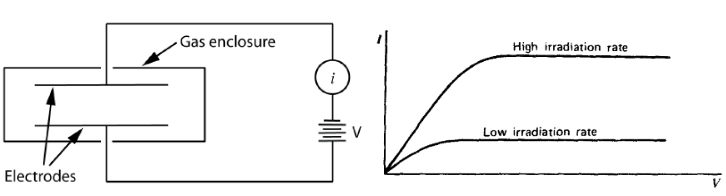
\includegraphics[scale=0.35]{ch8/image2}
	\captionof{figure}{ }
	\end{wrapfigure}
	Le principe est donc simple : un chambre, deux électrodes et un ampèremètre pour le courant. 
	En pratique, c'est plus compliqué car il faut gérer les courants de fuites. Notons que 
	les parois d'une chambre d'ionisation ainsi que les électrodes sont obligatoirement faits d'un
	matériau solide. Pour limiter les perturbations les électrodes sont en aluminium et les parois 
	en plastique (les matériaux les plus tissu-équivalents).
	

	\subsection{Configurations géométriques d'une chambre d'ionisation}
	Voir les deux slides traitant
	de la configuration géométrique de ces chambres, 48-49.

	\newpage		
	\subsection{Collection des charges}
	Celle-ci se fait en huit étapes
	\begin{enumerate}
	\item En moins de $10^{-7}$ s, $N_i$ paires sont produites
	\item Les électrons/ions subissent des collisions avec les atomes du gaz (diffusion/recombinaison, 
	attachement, transfert de charge).
	\item Les paires sont accélérées parallèlement au champ électrique
	\item Perte de la mémoire à chaque collision, puis ré-accéléré : le chemin suivi est une suite de
	chocs et d'accélérations
	\item Déplacement des charges combinaison de deux processus : diffusion (chocs avec les atomes)
	et migration (champ électrique).
	\item La vitesse de migration des ions $u_+$ est faible par rapport à celle des électrons $u_-$.
	\item La charge et le potentiel du condensateur évoluent jusqu'à la collection complète des
	charges au cours de la migration
	\end{enumerate}		

	\begin{center}
	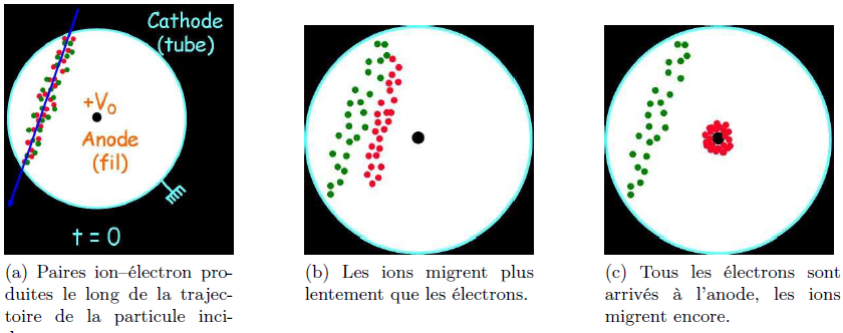
\includegraphics[scale=0.45]{ch8/image3}
	\captionof{figure}{Attention que, pour un gaz non électronégatif, il n'y a pas d'attachement.}
	\end{center}	
	
	Il ne faut pas imaginer que la collecte commence au moment où la charge arrive au condensateur.
	Dès qu'il y a séparation des charges, la collecte commence (charge induite dès l'apparition des
	charges et donc un signal). Ce signal induit à par contre peu d'influence en mode courant. 
	
	\subsection{Chambre d'ionisation en mode impulsion}		
	Les chambres d'ionisation en mode impulsion sont encore utilisées dans une certaine mesure en
	spectrométrie (bien qu'elles aient été largement remplacées par des détecteurs à 
	semiconducteur) et pour certaines applications très spécialisées comme des spectromètres $\alpha$
	à grande fenêtre d'entrée ou pour la détection de neutrons.\\
	
	Nous allons maintenant montrer le développement de l'impulsion. Considérons deux électrodes 
	planes et parallèles (distance $d$ entre-eux) et un gaz à faible coefficient d'attachement tel
	que l'électron est libre (il ne faut donc pas que le gaz contienne de l'O$_2$ sans quoi la forme
	du signal serait distordue). Ces deux électrodes forment un condensateur de capacité $C$ et un
	champ électrique constant et perpendiculaire aux électrodes est causé par une tension $U_0$.\\
	
	Lorsqu'une paire se crée, elle commence à dériver mais \underline{chaque charge induit une 
	charge image de même valeur absolue sur l'électrode} : un signal apparaît\textbf{dès} la création
	de la paire, bien avant la collecte. Les électrons arrivent à l'anode en $T_-$ et les ions 
	positifs en $T_+$, bien plus "grand" que $T_-$. Il résulte un courant impulsionnel formé de 
	deux contribution. Une rapide venant de l'électron et une lente du à l'ion positif.\\
	
	Le développement de la charge et du courant peut s'obtenir via le théorème de 
	\textsc{Ramo-Shockley}\footnote{Non démontré car très technique}\ \\
	
	\theor{\textsc{Ramo-Shockley}\ \\
	Soit $n$ électrodes dans un détecteur et $i_k$, le courant injecté dans une de ces électrodes
	durant le mouvement de la charge $q$ située entre les électrodes. Le courant injecté à 
	l'électrode vaut	
	\begin{equation}
	i_k=\frac{dQ_k}{dt}=q\vec{u}_q\vec{E}_k
	\end{equation}
	où $Q_k$ est la charge induite à l'électrode $k$, $\vec{u_q}=u_q\vec{1_q}$ est la vitesse de
	la charge $q$ et $\vec{E_k}$ est le champ électrique au point occupé par la charge $q$ quand
	l'électrode $k$ est à un potentiel de 1 V et que les autres électrodes sont à un potentiel 
	nul.}\ \\
	
	\begin{wrapfigure}[12]{l}{7cm}
	\vspace{-8mm}
	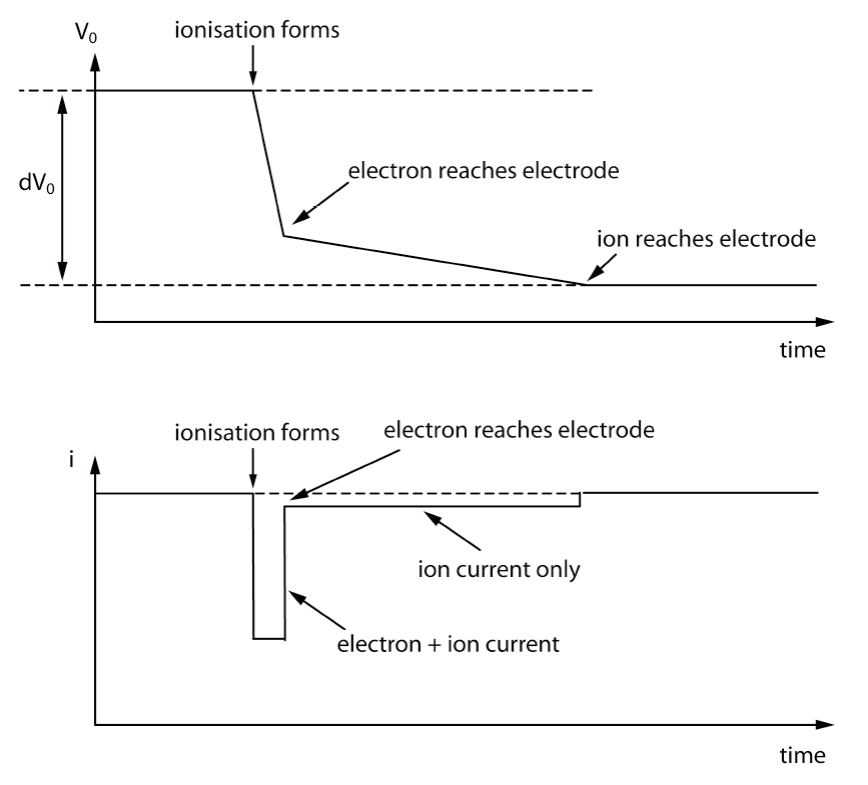
\includegraphics[scale=0.3]{ch8/image4}
	\captionof{figure}{ }
	\end{wrapfigure}
	
	Le courant à l'anode\footnote{Car charge induite opposée sur celle-ci} résultant est de $i_a=i_-
	+i_+$, pour un électron se déplaçant à $u_-$ vers l'anode et un ion à vitesse $i_+$ vers la
	cathode
	\begin{equation}
	i_-=-e\vec{u}_-\vec{E}_a=e\frac{u_-}{d},\qquad\qquad
	i_+=e\vec{u}_+\vec{E}_a=e\frac{u_+}{d}
	\end{equation}
	
	Si une paire est crée en $x=x_0$ en $t=0$, un courant$i_+$ apparaît jusqu'à s'annuler en 
	$T_+=x_0/u_+$ lorsque l'ion est collecté à la cathode mais aussi un courant $i_-$ qui 
	s'annule au temps $T_-=(d-x_0)/u_-$ lorsque l'électron est collecté par l'anode.\\
	\ \\
	\ \\

	\subsection{Chambre de Frish}
	En ajoutant une grille entre l'anode et la cathode, \textsc{Frish} propose une solution pour 
	supprimer l'influence de l'ion positif sur l'anode. En portant cette grille à un potentiel 
	entre 0 et $U_0$, elle sert d'écran électrostatique afin que l'anode ne soit influencée que
	par les charges entre elle-même et cette grille. Il n'y a plus aucune influence des ions
	puisqu'ils se déplacent uniquement dans l'espace compris entre la grille et la cathode, la
	largeur de l'impulsion est ainsi uniquement déterminée par le temps de collection des 
	électrons (et aussi par $\tau = RC$).

	
	\subsection{Résolution en énergie pour la chambre d'ionisation}
	Le facteur de \textsc{Fano} vaut $\pm$0.15 pour une chambre d'ionisation. Pour une particule
	$\alpha$ d'une énergie de 5.5 MeV totalement stoppée par un gaz ou $W=30$ eV, nous avons
	\begin{equation}
	N_i=\frac{E_{abs}}{W}=\frac{5.5\times 10^6}{30}=1.83\times 10^5 \mbox{paires}
	\end{equation}
	La résolution vaut alors
	\begin{equation}
	R=2.35\sqrt{\frac{F}{N_i}}=0.213\%
	\end{equation}
	Ce qui correspond à une largeur de raie de $R\times 5500$ keV = 11.7 keV.
	
\newpage
\section{Compteur proportionnel}%sl66	
Le signal produit par un rayonnement étant souvent trop petit que pour être observé, le compteur
proportionnel amplifie la charge \underline{\textbf{dans}} le gaz afin d'avoir un signal plus
important. On les utilise presque toujours en mode impulsion pour la détection/spectro des $\alpha$
et la détection des électrons mais également pour la spectrométrie des rayons $X$ de faible 
énergie (et la détection de neutrons).

\subsection{Champ électrique et potentiel dans le cylindre}	%sl68
	\begin{wrapfigure}[7]{l}{6cm}
	\vspace{-5mm}
	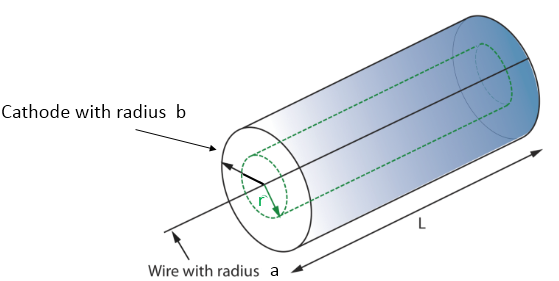
\includegraphics[scale=0.35]{ch8/image5}
	\captionof{figure}{ }
	\end{wrapfigure}
	
Considérons une géométrie cylindrique. A partir de $\int \vec{E} \vec{dS}=\frac{1}{\epsilon_0} \int q
dV$, on en tire (en négligeant les effets de bord)
\begin{equation}
E(r)2\pi rL=Q \Rightarrow E(r)=\frac{Q}{2\pi\epsilon_0 rL}
\end{equation}
Avec le champ électrique dans le cylindre $E=-\frac{dV}{dr}$ et en intégrant le long d'une ligne
radiale entre $a$ et $b$
\begin{equation}
V(b)-V(a)=\int_a^b E(r)dr
\end{equation}
En considérant le cylindre extérieur à la masse $V(b)=0$ et le fil central connecté à une alimentation
en tension externe telle que $V(a)=U_0$
\begin{equation}
U_0=\int_a^b E(r)dr=\frac{Q}{2\pi\epsilon_0 L}\ln{\left(\frac{b}{a}\right)}
\end{equation}
En éliminant $Q$
\begin{equation}
E(r)=\frac{U_0}{r\ln{b/a}}
\end{equation}

	\begin{wrapfigure}[6]{l}{6cm}
	\vspace{-15mm}
	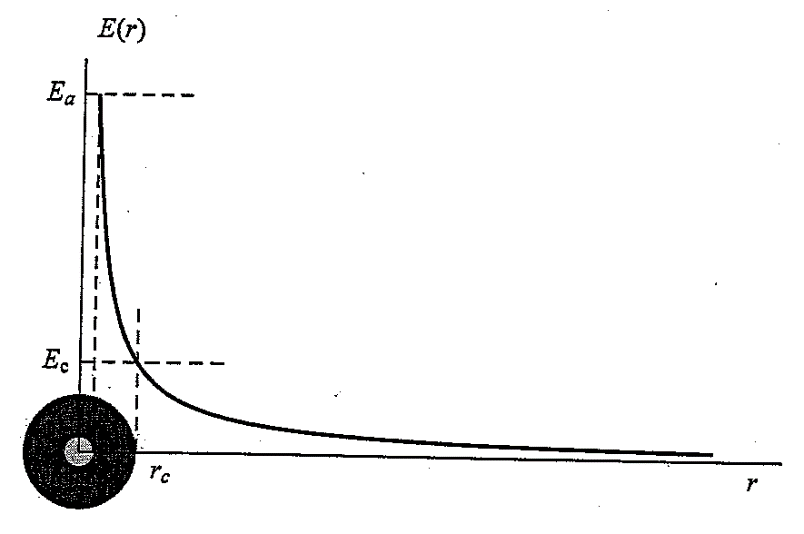
\includegraphics[scale=0.25]{ch8/image6}
	\captionof{figure}{ }
	\end{wrapfigure}
	
A cause de variation du champ en $r^{-1}$, les grandes valeurs du $E(r)$ ne sont obtenue qu'à
proximité du fil constituant l'anode. Il s'agit de la région de multiplication de rayon critique
$r_C$ dans laquelle règne un champ électrique plus grand que $E_C$ (champ pour lequel la
multiplication devient critique).



\subsection{Principe de multiplication}%sl71
On ne nous la fait plus : un rayonnement incident crée des paires qui vont migrer vers les
électrodes. A proximité de l'anode le champ augmente. Dans la zone de multiplication 
($\approx \mu m$), il y a multiplication de la charge. Les "nouveau" électrons ont assez 
d'énergie pour ioniser les atomes et créer à leur tour d'autres électrons : augmentation
exponentielle.\\

Par contre, l'ionisation se produit \textbf{exclusivement} dans la région de multiplication pour
tous les électrons primaires ($r_C$ est très petit, <0.2\% du volume total). Cette région n'est
donc \textbf{jamais} traversée par la particule initiale de sorte à ce que le gain du compteur
soit \textbf{indépendant} de la position de la trajectoire du rayonnement initial.\\

Un nombre égal d'électrons et ions sont crées (les électrons atteignent bien plus vite l'électrode
que les ions positifs) mais ces-derniers ne sont pas accélérés car le champ électrique n'est, pour 
eux, pas suffisament important.

\subsection{Collecte des charges}%sl75
La quasi-totalité des charges générées dans le compteur ont pour origine la région de multiplication, 
en ignorant donc totalement la position initiale de la paire. Le temps de collecte peut être divisé
en deux
\begin{enumerate}
\item Le temps de dérive $t_r$ (temps nécessaire à l'électron libre pour atteindre la région de
multiplication)
\item Le temps de multiplication $t_m$ (temps entre le début de l'avalanche et la collection 
complète)
\end{enumerate}
La contribution du signal est plus faible durant $t_r$ que $t_m$ de sorte que le temps de dérive
introduit juste un délai avant la mesure de l'impulsion. \\

Par contre, la quasi-totalité des ions et des électrons sont créés à proximité de l'anode, 
le signal mesuré est donc principalement dû à la dérive des ions plutôt qu'au mouvement des 
électrons\footnote{Pas clair. A mieux expliquer}. Initialement les ions sont soumis à un champ
électrique élevé : ils ont un mouvement rapide sans multiplication et donnent une impulsion à flanc rapide.


\subsection{Analyse simplifiée de la collecte des charges}%sl77
Soit un condensateur cylindrique de rayons interne $a$ et externe $b$ chargé via un potentiel 
$U_0$ formant un condensateur $C$. L'énergie absorbée parle mouvement d'une charge $Q$ positive le
long d'une distance $dr$ vaut
\begin{equation}
\frac{d\varepsilon}{dr}=QE(r)=Q\frac{U_0}{r\ln{(b/a)}}
\end{equation}
Supposons que $n_0$ ions et électrons soient formés dans l'avalanche à une distance $\rho$ de la
surface de l'anode ($Q=en_0$). Soit $U_{ch}$ la tension aux bornes de la chambre et $U_R$ aux bornes
de la résistance du circuit de mesure. L'énergie absorbée durant le mouvement des ions positifs vers
la cathode vaut
\begin{eqnarray}
\varepsilon^+&=&\int_{a+\rho}^{b}\frac{d\varepsilon}{dr}dr=\frac{QU_0}{\ln{(b/a)}}\int_{a+\rho}^{b}\frac{dr}{r}\\
&=&\frac{QU_0}{\ln{(b/a)}}\ln{\frac{b}{a+\rho}}
\end{eqnarray}
Même calcul pour les électrons
\begin{eqnarray}
\varepsilon^-&=&-\frac{QU_0}{\ln{(b/a)}}\int_{a+\rho}^{a}\frac{dr}{r}\\
&=&\frac{QU_0}{\ln{(b/a)}}\ln{\frac{a+\rho}{a}}
\end{eqnarray}
L'énergie totale absorbée après collection complète des deux types de charges vaut
\begin{eqnarray}
\Delta\varepsilon&=&\varepsilon^++\varepsilon^-=\frac{QU_0}{\ln{(b/a)}}\ln{\left(\frac{b}{a+\rho}\frac{a+\rho}{a}\right)}\\
&=&QU_0
\end{eqnarray}
Expression que l'on simplifie en $Q*U_0$, soit la charge multipliée par la différence de potentiel.
Par conservation de l'énergie, l'énergie restant dans le condensateur est l'énergie initiale à 
laquelle on soustrait l'énergie perdue durant le déplacement $\Delta \epsilon$
\begin{eqnarray}
&&\frac{CU_{ch}^2}{2}=\frac{CU_{0}^2}{2}-\Delta\varepsilon\\
&&\frac{C}{2}(U_{ch}-U_0)(U_{ch}+U_0)=-\Delta\varepsilon
\end{eqnarray}

	\begin{wrapfigure}[8]{r}{5.6cm}
	\vspace{-5mm}
	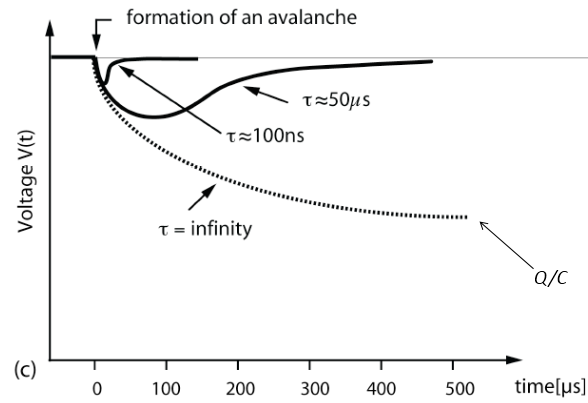
\includegraphics[scale=0.35]{ch8/image7}
	\captionof{figure}{ }
	\end{wrapfigure}

En supposant $\Delta\epsilon$ petit, $U_{ch}+U_0=2U_0$ et $U_R=U_0-U_{ch}$ de sorte à écrire
\begin{equation}
U_R=\frac{\Delta\varepsilon}{CU_0}=\frac{QU_0}{CU_0}=\frac{Q}{C}
\end{equation}
où $U_R$ est l'amplitude maximale mesurée mais il faut que $RC$ soit grand par rapport au temps 
de collection des ions. En pratique ce n'est jamais respecté et le maximum dépendra de $RC$.\\

Calculons le rapport des énergies absorbées durant le mouvement des électrons et des ions positifs
\begin{equation}
\frac{\varepsilon^-}{\varepsilon^+}=\frac{\ln{[(a+\rho)/a]}}{\ln{[b/(a +\rho)]}}
\end{equation}
Pour des paramètres réalistes, on trouve $\frac{\varepsilon^-}{\varepsilon^+}=0.019$ ce qui signifie
que moins de 2\% du signal résulte du mouvement des électrons : leur contribution est négligée. C'est
logique car les électrons sont proches du fil central et seront directement collectés (très 
rapidement) donc peut de contribution. L'avalanche est due au électrons mais le signal aux 
ions\footnote{Je comprends l'idée, mais quelque chose m'échappe physiquement. En quoi les ions 
contribuent plus au signal que les électrons? Car ils parcours moins de distances et donc leur 
énergie est moins absorbée?}

\subsection{Temps de multiplication pour les ions}%sl83
On s'intéresse ici au temps entre l'avalanche et la collecte de charge. La vitesse de dérive de
l'ion est donnée par
\begin{equation}
u^+(r)=\mu E(r)=\mu\frac{U_0}{\ln{(b/a)}}\frac{1}{r}
\end{equation}
La position des ions s'obtient par
\begin{equation}
\int_a^{r(t)}\frac{dr'}{u^+(r')}=\int_0^{t}dt' \Rightarrow r(t)=\left(2\mu\frac{U_0}{\ln{(b/a)}}t+a^2\right)^{1/2}
\end{equation}
Le temps de multiplication $t_m$ s'obtient via $r(t)=b$
\begin{equation}
t_m=\frac{(b^2-a^2)\ln{(b/a)}}{2\mu U_0}
\end{equation}
La valeur typique est de quelques centaines de microsecondes, le temps que les ions franchissent
toute la distance. Ce temps est long, mais une large fraction du signal se développe durant la
première partie de la dérive des ions. Il faut donc regarder l'énergie absorbée durant le 
mouvement des ions en fonction du temps 
\begin{equation}
\varepsilon^+(t)=\frac{QU_0}{\ln{(b/a)}}\int_a^{r(t)}\frac{dr'}{r'}=\frac{QU_0}{\ln{(b/a)}}\ln{\frac{r(t)}{a}}
\end{equation}
En y substituant l'expression de $r(t)$ et celle de $U_R(t) = \epsilon^+/CU_0$, on peut écrire
\begin{equation}
U_R(t)=\frac{Q}{C\ln{(b/a)}}\ln{\left(\frac{2\mu U_0}{a^2\ln{(b/a)}}t+1\right)^{1/2}}
\end{equation}
L'impulsion atteint la moitié de son impulsion pour un temps
\begin{equation}
t_{1/2}=\frac{a}{a+b}t_m
\end{equation}
Avec des données réalistes, $t_{1/2}/t_m = 0.25\%$ : augmentation rapide de l'impulsion et ensuite
croissance plus lente qui ne contribuera plus à l'amplitude du signal. Notons que la dérive $t_r$
introduit une dispersion temporelle détériorant la résolution.\footnote{Il ne faut pas savoir 
refaire ces expressions mais l'ordre de grandeur, l'expression $t_{1/2}$, \dots il faut connaître.}
\begin{center}
	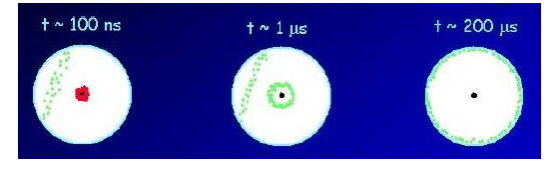
\includegraphics[scale=0.5]{ch8/image8}
	\captionof{figure}{Initialement les ions ne bougent pas, les électrons sont directement collectés
	après une multiplication sur un temps très court puis les ions migrent pour être collectés. Les
	ions venant du passage de la particule chargée ne contribuent quasiment pas.}
\end{center}

\subsection{Équation de Townsend}%sl87

	\begin{wrapfigure}[10]{l}{4cm}
	\vspace{-5mm}
	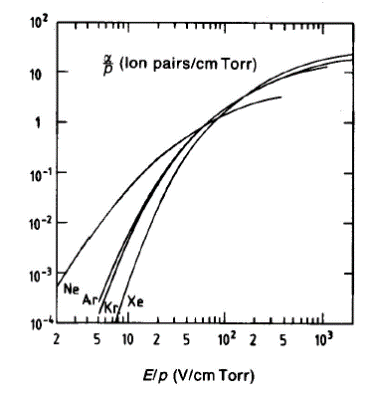
\includegraphics[scale=0.35]{ch8/image9}
	\captionof{figure}{ }
	\end{wrapfigure}
La probabilité pour un électron de créer un électron additionnel sur $dx$ est de $\alpha dx$ où
$\alpha$ est le premier coefficient de \textsc{Townsend}. Le processus de multiplication est
régit par l'équation de \textsc{Townsend} qui donne la variation relative du nombre d'électrons
$n(x)$ par unité de longueur parcourue
\begin{equation}
\frac{dn}{n}=\alpha dx {\mbox{~~avec~~}}\alpha=0  {\mbox{~~pour~~}}E<E_c
\end{equation}
où $\alpha$ dépend des section efficaces, du champ électrique et de la densité du gaz.



\subsection{Expression mathématique du coefficient de multiplication}%sl89
Pour $E>E_C$,le nombre d'électron croît donc exponentiellement avec la distance parcourue
\begin{equation}
n(x)=n(0)\exp{(\alpha x)} {\mbox{~~pour~~}}E>E_c
\end{equation}
On \textbf{définit} le coefficient de multiplication du compteur (le \textit{gain} du compteur) par
$M=n(x)/n(0)$ ce qui donne
\begin{equation}
{\mbox{pour~~}}a<x<r_c \Rightarrow \ln{M}=\int_a^{r_c}\alpha(x)dx=\int_{E_a}^{E_c}\frac{\alpha(E)}
{(dE/dx)}dE
\end{equation}
Il n'existe pas d'expression pour $\alpha(E)$, mais pour $E$ "pas trop grand" $\alpha(E)=\beta E$.
En intégrant
\begin{eqnarray}
\ln{M}&=&\beta\frac{U_0}{\ln{(b/a)}}\ln{\frac{E(a)}{E_c}}=\beta\frac{U_0}{\ln{(b/a)}}\ln{\frac{r_c}{a}}\\
&=&\beta\frac{U_0}{\ln{(b/a)}}\ln{\frac{U_0}{E_ca\ln{(b/a)}}}
\end{eqnarray}

\subsection{Paramètres de Diethorn}
Il est possible de calculer $M$ d'une autre façon, sachant que la différence de potentiel entre
l'anode ($r=a$) et le rayon critique ($r=r_C$) vaut
\begin{equation}
V(a)-V(r_c)=\frac{U_0}{\ln{(b/a)}}\ln{\frac{r_c}{a}}
\end{equation}
Si $e\Delta V$ est l'énergie moyenne nécessaire pour produire un électron supplémentaire, le nombre
de désintégration $Z$ vaut
\begin{equation}
Z=\frac{V(a)-V(r_c)}{\Delta V}
\end{equation}
Pour le gain
\begin{equation}
M=2^Z\Rightarrow \ln{M}=\ln{2}Z=\frac{\ln{2}}{\Delta V}\frac{U_0}{\ln{(b/a)}}\ln{\frac{r_c}{a}}
\end{equation}
En supposant que $E_C\propto\rho, E_C(\rho) = E_C(\rho_0)\rho/\rho_0$ est l'expression de 
\textsc{Diethorn} pour $M$
\begin{equation}
\ln{M}=\frac{\ln 2}{\Delta V}\frac{U_0}{\ln{b/a}}\ln{\frac{\rho_0U_0}{\rho E_c(\rho_0) a\ln{b/a}}}
\end{equation}
où $\Delta V$ et $E_C(\rho_0)$ sont obtenus par comparaison avec les données expérimentales. Sans
les connaître, on en déduit que
\begin{equation}
\frac{\ln{b/a}}{U_0}\ln{M}\propto \ln{\frac{\rho_0U_0}{\rho E_c(\rho_0) a\ln{b/a}}}
\end{equation}


\subsection{Choix du gaz}%sl96
Il ne faut \textbf{jamais} que le gaz contienne un composant électronégatif formant des ions
négatifs qui ne seraient pas accélérés. L'air est à bannir, les gaz nobles constituent un bon 
choix. L'argon est souvent retenu car bon marché. Par contre, les gaz nobles ont plusieurs 
problèmes :
\begin{enumerate}
\item Il peut y avoir des ionisations mais aussi des excitations se manifestant par après par
l'émission d'UV. Le gaz peut l'absorber, émettre un électron et relancer l'avalanche. 
\item La recombinaison induit aussi es UV
\item L'énergie moyenne des gaz noble est élevée et peut donner des UV pouvant extraire un électron
de la cathode relançant l'avalanche.
\item Les ions positifs du gaz vont se neutraliser par l'extraction d'un électron de la cathode.
L'énergie dissipée peut extraire un électron additionnel et relancer l'avalanche.
\end{enumerate}\ 


	\begin{wrapfigure}[10]{l}{5cm}
	\vspace{-7mm}
	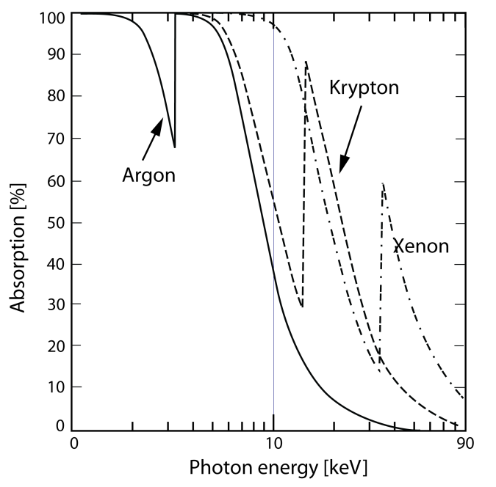
\includegraphics[scale=0.35]{ch8/image10}
	\captionof{figure}{ }
	\end{wrapfigure}

Heureusement il existe une solution : ajouter ($\approx10\%$) un gaz de \textit{quenching} (coupure)
possédant de nombreux degrés de libertés de rotation et vibration afin d'absorber les UV et 
assurer le transfert de charge Ar$^+$ + gaz $\to$ Ar + gaz$^+$.\\
	
Pour les rayons $X$, l'Ar n'est pas le meilleur choix car la probabilité d'interaction des photons 
diminue fortement pour des énergies supérieurs à 20 keV. On utilisera alors du Kr et Xe qui donne
une efficacité raisonnable jusqu'à 100 keV.\\

Notons que si $N_i$ est trop important, la charge d'espace qu'ils représentent peut perturber le
champ électrique ce qui cause une perte de la résolution suivie d'une perte de 
proportionnalité.



\newpage
\subsection{Résolution du détecteur}%sl100
Soit $Q$, la charge collecté par le compteur proportionnel (sans effets non-linéaires), $N_i$ le
nombre de paires et $M$ le facteur de multiplication tel que (sans recombinaisons)
\begin{equation}
\langle Q \rangle = e\langle N_i \rangle \langle M \rangle
\end{equation}
Si $N_i$ et $M$ sont indépendants,la variance sur $Q$ est donnée par
\begin{equation}
\left(\frac{\sigma_{Q_{}}}{Q}\right)^2=\left(\frac{\sigma_{N_{i}}}{N_i}\right)^2+\left(\frac{\sigma_{M_{}}}{M}\right)^2
\end{equation}
On considère généralement la variance sur $A$, le facteur de multiplication pour \textit{un seul}
électron initialement crée
\begin{equation}
M=\frac{1}{N_i}\sum_{i=1}^{N_i}A_i\equiv\bar{A}
\end{equation}
Les avalanches pour chaque électron étant indépendantes
\begin{equation}
\sigma_M^2=\left(\frac{1}{N_i}\right)^2\sum_{i=1}^{N_i}\sigma_A^2=\frac{1}{N_i}\sigma_A^2
\end{equation}
La variance sur $Q$ devient
\begin{equation}
\left(\frac{\sigma_{Q_{}}}{Q}\right)^2=\left(\frac{\sigma_{N_{i}}}{N_i}\right)^2+\frac{1}{N_i}\left(\frac{\sigma_{A}}{\bar{A}}\right)^2
\end{equation}
Pour tenir compte des variation sur $N_i$, on introduit le facteur de \textsc{Fano}
\begin{equation}
\left(\frac{\sigma_{N_{i}}}{N_i}\right)^2=\frac{F}{N_i}
\end{equation}
Pour les variations sur $A$, plusieurs modèles :
\begin{description}
\item[Distribution de \textsc{Furry}] 
\begin{equation}
P(A)=\frac{(1-1/\bar{A})^{A-1}}{\bar{A}}
\end{equation}
\item[Distribution de \textsc{Furry} pour $A$ grand]
\begin{equation}
P(A)=\frac{e^{-A/\bar{A}}}{\bar{A}}
\end{equation}
Dans ce cas
\begin{equation}
\left(\frac{\sigma_A}{\bar{A}}\right)^2=1
\end{equation}
Expérimentalement ceci n'est pas vérifié. On introduit alors la distribution de \textsc{Polya}.
\item[Distribution de \textsc{Polya}]
\begin{equation}
P(A)=\left[\frac{A(1+\theta)}{\bar{A}}\right]^\theta\exp{\left[\frac{-A(1+\theta)}{\bar{A}}\right]}
\end{equation}
Dans ce cas (pour de grandeurs valeurs de $\bar A$
\begin{equation}
\left(\frac{\sigma_A}{\bar{A}}\right)^2=\frac{1}{\bar{A}}+b\simeq b
\end{equation}
où $b=1/(1+\theta)$.
\end{description}
Pour les variations sur $Q$
\begin{equation}
\left(\frac{\sigma_{Q}}{Q}\right)^2=\frac{F}{N_i}+\frac{b}{N_i},\qquad\qquad
\left(\frac{\sigma_{Q}}{Q}\right)^2=\frac{1}{N_i}(F+b)
\end{equation}
La fluctuation sur l'avalanche domine. On note aussi cette équation en considérant $N_i=E/W$
\begin{equation}
\frac{\sigma_{Q}}{Q}=\left[\frac{W(F+b)}{E}\right]^{1/2}
\end{equation}



\subsection{Pic d'échappement et compteur proportionnel multi-fils}%sl107
\subsubsection{Pic d'échappement}
	\begin{wrapfigure}[10]{r}{6cm}
	\vspace{-5mm}
	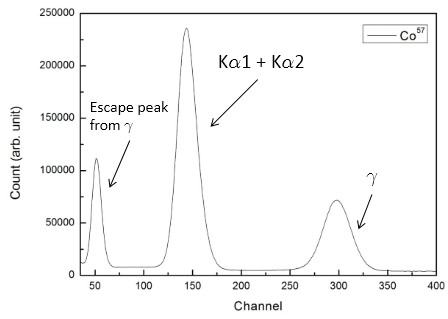
\includegraphics[scale=0.5]{ch8/image11}
	\captionof{figure}{ }
	\end{wrapfigure}
Parfois on observe un pic d'échappement : une énergie précise s'est échappée. Après un effet
photoélectrique (par un rayonnement $X$ initial tel que $E_{RX} > B_K$), un 
électron de la couche $K$ est émis. Par réarrangement électronique, un rayon $X$ d'énergie
$B_K-B_L$ peut s'échapper. S'il s'échappe, celui-ci aura l'énergie $E_{RX}-(B_K-B_L)$. S'il
est détecté, il en résultera un pic d'absorption total.	\\
\ \\

Si l'énergie initial du $X$ est tel que $B_L<E_{RX}<B_K$, un électron de la couche $L$ est émis
et, par réarrangement électronique, un $X$ d'énergie $B_L-B_M$ ne pouvant s'échapper (énergie
trop faible). 
	
\subsubsection{Compteur proportionnel multi-fils pour la détection de traces}
Il s'agit de deux cathodes planes avec une série de fils d'anodes entre les plans cathodiques. Le 
champ électrique est similaire à celui précédemment décrit mais cette géométrie permet d'avoir des
informations sur la trajectoire des particules incidentes.
	
	
\section{Compteur Geiger}%sl110	
Ce détecteur a été développé en \textit{1928} par \textsc{Geiger} et \textsc{Müller} et est toujours
utilisé aujourd'hui (simplicité, faible coût et facilité d'utilisation). Pour avoir un tel 
compteur, il faut $U_0$ élevé pour avoir une probabilité d'excitation des molécules de gaz élevée
et donc une probabilité d'émission de photons UV élevé de sorte que la probabilité d'absorption 
par rapport à l'effet photoélectrique soit élevé pour avoir émission d'un électron. Le but est
que chaque avalanche en produise au moins une autre de sorte à avoir une réaction en chaîne (décharge)
maintenue par les rayonnements UV.\\

A cause des ions positifs, la décharge va s'arrêter (une concentration élevée diminue le champ 
électrique au voisinage de l'anode à une valeur inférieure à $E_C$). Ceux-ci ayant une faible
mobilité, ils vont être essentiellement au repos le temps que les électrons soient collectés. Pour
une tension $U_0$, la décharge se stoppe ainsi toujours après le développement de la même valeur de
charge totale. Il y a donc indépendance par rapport au nombre de paires d'ions crées par le 
rayonnement initial : le compteur \textsc{Geiger} n'est qu'un compteur de particules.
	
	
	
\subsection{Gaz de quenching}%sl113
Après la décharge, les ions positifs arrivent à la cathode où ils se neutralisent et libérer une
énergie. Si cette énergie arrache un électron, elle peut relancer une avalanche. La probabilité que
ça arrive est faible mais il y a tellement d'ion que ça se produit. Le problème est que ça recommence
un comptage ce qu'il faut éviter.\\

On va alors ajouter un gaz de quenching pour que les ions subissent des collision avec les molécules
de ce gaz : tous les ions primaires seront neutralisés en transférant la charge positive au gaz de 
quenching. Les ions du gaz de quenching arrivent alors à la cathode pour se faire neutraliser mais
l'énergie excédentaire va prioritairement induire la dissociation de la molécule et ainsi éviter
l'avalanche additionnelle. Le compteur a ainsi un temps de vie limité. Pour eviter ça, on utilise
du Cm$_2$ ou du Br$_2$ qui se recombinent après un certain temps pour avoir un temps de vie 
illimité (théoriquement, mais d'autres effets limitent sa durée de vie).


\subsection{Collection des charges}%sl116
Le principe est le même que pour un compteur proportionnel mais un peu plus complexes : les avalanches
se forment tout au long de l'anode mais ce qui complexifie est la modification du champ électrique
à cause des charges d'espace. Le temps de collecte est un peu plus long que pour une avalanche
unique et dépendra du produit $RC$.

\subsection{Temps mort et temps de restitution}%sl118
L'accumulation de charge causant l'arrêt de la décharge ne permet pas de générer une nouvelle 
décharge. La migration de la charge positive permet au champ de redépasser la valeur critique. La
détection est possible, mais d'amplitude plus faible. Le retour "complet" à la normal nécessite 
d'attendre le \textit{temps de restitution} de l'ordre de la miliseconde.


\subsection{Détection des $\gamma$}%sl120
Avec une fenêtre d'entrée mince, ils détectent les $\alpha$ (rarement) et les $\beta$ mais ils servent
surtout à la détection des $\gamma$ qui, quand ils interagissent avec la paroi, produit des électrons
par effet photoélectrique ou \textsc{Compton}. Les électrons quittant la paroi pénètrent dans le
gaz et donnent lieu à des ionisation constituant le signal du compteur.\\

L'efficacité pour détecter des $\gamma$ dépend de deux choses 
\begin{enumerate}
\item La probabilité que le $\gamma$ interagisse avec la paroi et produise un électron
\item La probabilité que l'électron atteigne le gaz avant la fin de son parcours (dépendra du travail
d'extraction du matériau constituant la paroi)
\end{enumerate}
Seul la couche laplus interne de la paroi contribue à la production d'électron. Cette région a une épaisseur équivalente au range maximum des electrons créés dans la paroi et, dès lors, augmenter
l'épaisseur ne va pas augmenter l'efficacité (mais au contraire diminuer par absorption des 
$\gamma$ dans les couches externes de la paroi). La probabilité d'interaction augmente parcontre
lorsque $Z$ augmente.
	







